\newpage
\section{Autenticazione}

\label{Autenticazione}
\begin{figure}[ht]
	\centering
	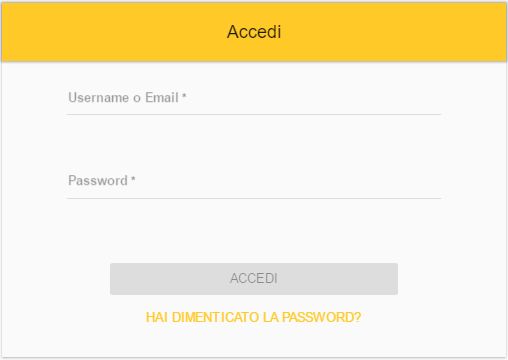
\includegraphics[scale=0.65]{img/autenticazione.png}
	\caption{Autenticazione}
\end{figure}
\FloatBarrier

Effettuata la registrazione è possibile autenticarsi al sistema. Compilati correttamente i campi \textit{Username o E-mail} e \textit{Password} il bottone \textit{Accedi} viene abilitato dando la possibilità di autenticarsi. Se l'utente non ricorda più la propria password personale è possibile cliccare sulla stringa \textit{HAI DIMENTICATO LA PASSWORD?} per recuperarla. Verrà presentata la seguente pagina:

\label{RecuperoPassword}
\begin{figure}[ht]
	\centering
	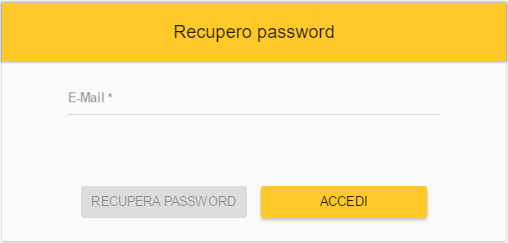
\includegraphics[scale=0.48]{img/recupero_password.png}
	\caption{Recupero Password}
\end{figure}
\FloatBarrier

la quale permette di recuperare la password inserendo la propria mail nell'apposito campo. La password sarà all'interno della mail che il sistema invierà all'indirizzo di posta elettronica inserito.  